\section{Sequences}

%%%%%%%%%%%%%%%%
%  Definition  %
%%%%%%%%%%%%%%%%

\subsection{Definition}

\Definition{Sequence}{
    A \textbf{sequence} is a function whose domain is the set of natural numbers $\mathbb{N}$. The sequence is denoted by $\{a_n\}$ and the value of the function at $n$ (the $n$-th term) is denoted by $a_n$. \\ 
    Various ways of representing a sequence are:
    \[ \{a_1, a_2, \dots, a_n, a_{n+1}, \dots\} \qquad \{a_n\} \qquad \{a_n\}_{n=1}^{\infty} \]
}


%%%%%%%%%%%%%%%%%%%%%%%%%%%%%%%%%
%  Precise Definition of Limit  %
%%%%%%%%%%%%%%%%%%%%%%%%%%%%%%%%%

\subsection{Precise Definition of Limit of a Sequence}

\Note[Precise Definition of Limit]{
    \begin{enumerate}
        \item We say that \[ 
                \lim_{n \to \infty} a_n = L
                \] if \[ 
                \forall \epsilon > 0, \exists N \in \N : \forall n \geq N, |a_n - L| < \epsilon
            \]
        \item We say that \[ 
                \lim_{n \to \infty} a_n = \infty 
                \] if \[ 
                \forall M \in \R, \exists N \in \N : \forall n \geq N, a_n > M
            \]
        \item We say that \[ 
                \lim_{n \to \infty} a_n = -\infty
                \] if \[ 
                \forall M \in \R, \exists N \in \N : \forall n \geq N, a_n < M
            \]
    \end{enumerate}
}


%%%%%%%%%%%%%%%%%%%%%%%%%%%%%%
%  Convergence of Sequences  %
%%%%%%%%%%%%%%%%%%%%%%%%%%%%%%

\subsection{Convergence of Sequences}
\Theorem{Convergence of Sequences}{
    A sequence $\left\{ a_n \right\}$ is said to be \textbf{convergent} if there exists a real number $L$ such that \[ 
        \lim_{n \to \infty} a_n = L
    \]
}

\Theorem{Uniqueness of Limits}{
    If a sequence $\left\{ a_n \right\}$ converges, then its limit is unique.
}

\Theorem{}{
    Given the sequence $\left\{ a_n \right\}$ if we have a function $f(x)$ such that $f(n) = a_n$ and $\displaystyle \lim_{x \to \infty} f(x) = L$ then $\displaystyle \lim_{n \to \infty} a_n = L$.
}

\Note[Properties of Convergent Sequences]{
    If $\left\{ a_n \right\}$ and $\left\{ b_n \right\}$ are both convergent sequences, then:
    \begin{enumerate}
        \item
            \[
                \lim_{n \to \infty} (a_n \pm b_n) = \lim_{n \to \infty} a_n \pm \lim_{n \to \infty} b_n
            \]
        \item
            \[
                \lim_{n \to \infty} ca_n = c \lim_{n \to \infty} a_n
            \]
        \item
            \[
                \lim_{n \to \infty} (a_n b_n) = \left( \lim_{n \to \infty} a_n \right)\left( \lim_{n \to \infty} b_n \right)
            \]
        \item
            \[
                \lim_{n \to \infty} \frac{a_n}{b_n} = \dfrac{\lim_{n \to \infty} a_n}{\lim_{n \to \infty} b_n}
                , \qquad \text{ provided } \lim_{n \to \infty} b_n \neq 0
            \]
        \item
            \[
                \lim_{n \to \infty} a_n^p = \left[ \lim_{n \to \infty} a_n \right]^p
                , \qquad \text{ provided } a_n \geq 0
            \]
    \end{enumerate}
}

\Theorem{Squeeze Theorem for Sequences}{
    If $\left\{ a_n \right\}$, $\left\{ b_n \right\}$ and $\left\{ c_n \right\}$ are sequences such that $a_n \leq b_n \leq c_n$ for all $n \geq N$ and $\displaystyle \lim_{n \to \infty} a_n = \lim_{n \to \infty} c_n = L$ then $\displaystyle \lim_{n \to \infty} b_n = L$.
}

\Theorem{}{
    \[ \text{If} \lim_{n \to \infty} \lvert a_n \rvert = 0, \text{ then } \lim_{n \to \infty} a_n = 0 \]
}

\underline{\textbf{Proof:}} \\ 
The main thing to this proof is to note that, \[ 
    -\lvert a_n \rvert \leq a_n \leq \lvert a_n \rvert
\]
Then note that, \[ 
    \lim_{n \to \infty} -\lvert a_n \rvert = -\lim_{n \to \infty} \lvert a_n \rvert = 0
\]
We then have that, \[ 
    0 \leq \lim_{n \to \infty} a_n \leq 0 
    \] and so by the Squeeze Theorem, \[ 
    \lim_{n \to \infty} a_n = 0 
\]

\Theorem{Convergent Sequences are Bounded}{
    If a sequence $\left\{ a_n \right\}$ is convergent, then it is bounded.
}

\Example{
    Determine if the following sequences converge or diverge: \\
    \textbf{1} $\left\{ \dfrac{n^2}{2n^2 + 1} \right\}$ \\
    \textbf{2} $\left\{ \dfrac{(-1)^n}{n} \right\}$ \\
    \textbf{3} $\left\{ \dfrac{n!}{n^n} \right\}$
}{
    \begin{enumerate}
        \item We can use the theorem about converting sequences to functions. Let $f(x) = \dfrac{x^2}{2x^2 + 1}$. Then \[ 
                \lim_{x \to \infty} \frac{x^2}{2x^2 + 1} = \lim_{x \to \infty} \frac{1}{2 + 1/x^2} = \frac{1}{2}
            \] Therefore, $\displaystyle \lim_{n \to \infty} \dfrac{n^2}{2n^2 + 1} = \frac{1}{2}$ and the sequence converges.
        \item Note that $\left| \dfrac{(-1)^n}{n} \right| = \dfrac{1}{n} \to 0$ as $n \to \infty$. By the theorem about absolute values, $\displaystyle \lim_{n \to \infty} \dfrac{(-1)^n}{n} = 0$ and the sequence converges.
        \item For large $n$, $n! = n \cdot (n-1) \cdot (n-2) \cdots 2 \cdot 1$ grows much slower than $n^n = n \cdot n \cdot n \cdots n \cdot n$. We have \[ 
                0 < \frac{n!}{n^n} = \frac{n}{n} \cdot \frac{n-1}{n} \cdot \frac{n-2}{n} \cdots \frac{2}{n} \cdot \frac{1}{n} \leq \frac{n}{n} \cdot \frac{n}{n} \cdot \frac{1}{n} = \frac{1}{n}
            \] Since $\displaystyle \lim_{n \to \infty} 0 = 0$ and $\displaystyle \lim_{n \to \infty} \frac{1}{n} = 0$, by the Squeeze Theorem, $\displaystyle \lim_{n \to \infty} \frac{n!}{n^n} = 0$ and the sequence converges.
    \end{enumerate}
    \begin{center}
        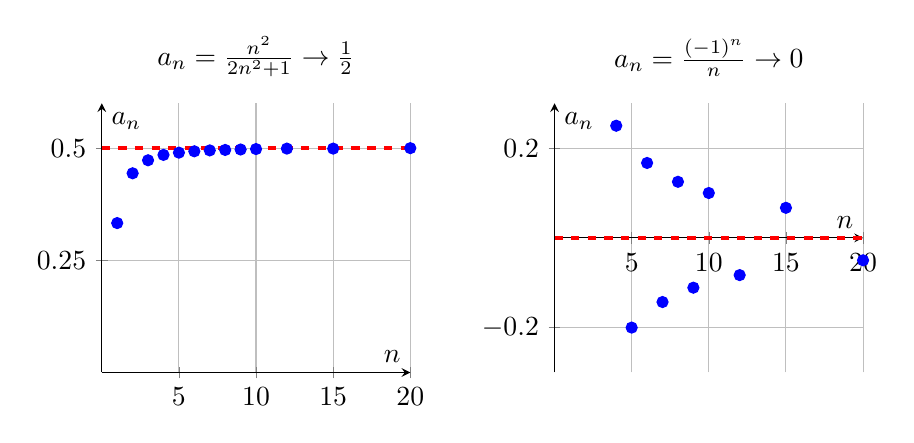
\begin{tikzpicture}
    % Sequence 1: n^2/(2n^2+1) -> 1/2
            \begin{axis}[
                name=seq1,
                width=5.5cm, height=5cm,
                axis lines=center,
                xlabel=$n$, ylabel=$a_n$,
                xmin=0, xmax=20,
                ymin=0, ymax=0.6,
                ytick={0,0.25,0.5},
                grid=major,
                title={$a_n = \frac{n^2}{2n^2+1} \to \frac{1}{2}$}
                ]
        % Limit line
                \addplot[red, dashed, very thick, domain=0:20] {0.5};
        % Sequence terms
                \addplot[blue, only marks, mark=*, mark size=2pt] coordinates {
                        (1,0.333) (2,0.444) (3,0.473) (4,0.485) (5,0.490) 
                        (6,0.493) (7,0.495) (8,0.496) (9,0.497) (10,0.498)
                        (12,0.499) (15,0.499) (20,0.500)
                    };
            \end{axis}
    % Sequence 2: (-1)^n/n -> 0
            \begin{axis}[
                at={(seq1.right of south east)}, anchor=left of south west,
                xshift=0.5cm,
                width=5.5cm, height=5cm,
                axis lines=center,
                xlabel=$n$, ylabel=$a_n$,
                xmin=0, xmax=20,
                ymin=-0.3, ymax=0.3,
                ytick={-0.2,0,0.2},
                grid=major,
                title={$a_n = \frac{(-1)^n}{n} \to 0$}
                ]
        % Limit line
                \addplot[red, dashed, very thick, domain=0:20] {0};
        % Sequence terms (alternating)
                \addplot[blue, only marks, mark=*, mark size=2pt] coordinates {
                        (1,-1) (2,0.5) (3,-0.333) (4,0.25) (5,-0.2) 
                        (6,0.167) (7,-0.143) (8,0.125) (9,-0.111) (10,0.1)
                        (12,-0.083) (15,0.067) (20,-0.05)
                    };
            \end{axis}
        \end{tikzpicture}
        \captionof{figure}{Sequence Convergence: Terms approach their limits as $n \to \infty$}
    \end{center}
}


\Theorem{}{
    For the sequence $\left\{ a_n \right\}$ if both $\displaystyle \lim_{n \to \infty} a_{2n} = L$ and $\displaystyle \lim_{n \to \infty} a_{2n+1} = L$, then $\left\{ a_n \right\}$ is convergent and $\displaystyle \lim_{n \to \infty} a_n = L$.
}

\Theorem{}{
    The sequence $\left\{ r^n \right\}_{n=0}^{\infty}$ converges if $-1 < r \leq 1$ and diverges for all other values of $r$. Also, \[
        \lim_{n \to \infty} r^n
        \begin{cases}
            0, &\text{ if } -1 < r < 1 \\
            1, &\text{ if } r = 1
        \end{cases}
    \]
}

\Theorem{}{
    For the sequence $\left\{ a_n \right\}$ if both $\displaystyle \lim_{n \to \infty} a_{2n} = L$ and $\displaystyle \lim_{n \to \infty} a_{2n+1} = L$, then $\left\{ a_n \right\}$ is convergent and $\displaystyle \lim_{n \to \infty} a_n = L$.
}

\underline{\textbf{Proof:}}  \\ 
Let $\epsilon > 0$. Then since $\displaystyle \lim_{n \to \infty} a_{2n} = L$, \[ 
    \exists N_1 \in \N : \forall n \geq N_1, \lvert a_{2n} - L \rvert < \epsilon
\]
Similarly, because $\displaystyle \lim_{n \to \infty} a_{2n+1} = L$, \[ 
    \exists N_2 \in \N : \forall n \geq N_2, \lvert a_{2n+1} - L \rvert < \epsilon
\]
Now, let $N = \max\{2N_1, 2N_2+1\}$ and let $n > N$. Then either $a_n = a_{2k}$ for some $k > N_1$ or $a_n = a_{2k+1}$ for some $k > N_2$, And so in either case we have that \[ 
    \lvert a_n - L \rvert < \epsilon
\]
Therefore, $\displaystyle \lim_{n \to \infty} a_n = L$ and so $\left\{ a_n \right\}$ is convergent.


%%%%%%%%%%%%%%%%%%%%%%%%%%%%%%%%%%%%%
%  Bounded and Monotonic Sequences  %
%%%%%%%%%%%%%%%%%%%%%%%%%%%%%%%%%%%%%

\subsection{Bounded and Monotonic Sequences}

\Definition{Bounded Sequence}{
    A sequence $\left\{ a_n \right\}$ is \textbf{bounded} if \[ 
        \exists M \in \R : \forall n \in \N, \lvert a_n \rvert \leq M
    \]
}

\Note[Upper and Lower Bounds]{
    If \[
        \exists m \in \R : \forall n \in \N, m \leq a_n
        \] the sequence $\left\{ a_n \right\}$ is said to be \textbf{bounded below} and $m$ is a \textbf{lower bound} of the sequence. Similarly, if \[
        \exists M \in \R : \forall n \in \N, M \geq a_n
    \] the sequence $\left\{ a_n \right\}$ is said to be \textbf{bounded above} and $M$ is an \textbf{upper bound} of the sequence.
}

\Theorem{Bounded Sequence}{
    If a sequence $\left\{ a_n \right\}$ is both bounded above and below, then it is bounded. That is, if \[ 
        \exists m, M \in \R : \forall n \in \N, m \leq a_n \leq M
    \] then $\left\{ a_n \right\}$ is bounded.
}

\Example{
    Determine if the following sequences are bounded: \\
    \textbf{1} $\left\{ \dfrac{\sin(n)}{n} \right\}$ \\
    \textbf{2} $\left\{ (-1)^n n \right\}$ \\
    \textbf{3} $\left\{ \dfrac{2n}{n+1} \right\}$
}{
    \begin{enumerate}
        \item Since $-1 \leq \sin(n) \leq 1$ for all $n$, and $n > 0$ for all $n \in \N$, we have \[ 
                -\frac{1}{n} \leq \frac{\sin(n)}{n} \leq \frac{1}{n}
            \] For $n \geq 1$, this gives us $-1 \leq \frac{\sin(n)}{n} \leq 1$. Therefore, the sequence is bounded with $m = -1$ and $M = 1$.
        \item The terms of this sequence alternate: $-1, 2, -3, 4, -5, 6, \dots$. As $n$ increases, $|(-1)^n n| = n$ grows without bound. Therefore, the sequence is unbounded.
        \item We can rewrite $\dfrac{2n}{n+1} = \dfrac{2n + 2 - 2}{n+1} = \dfrac{2(n+1) - 2}{n+1} = 2 - \dfrac{2}{n+1}$. Since $n \geq 1$, we have $\dfrac{2}{n+1} \leq \dfrac{2}{2} = 1$, so $a_n \geq 2 - 1 = 1$. Also, since $\dfrac{2}{n+1} > 0$, we have $a_n < 2$. Therefore, $1 \leq a_n < 2$ for all $n$, and the sequence is bounded.
    \end{enumerate}
}

\Definition{Monotonic Sequence}{
    A sequence $\left\{ a_n \right\}$ is \textbf{monotonic} if for all $n \in \N$ \[ 
        a_{n+1} \geq a_n \quad \text{or} \quad a_{n+1} \leq a_n
    \]
}

\Theorem{}{
    If a sequence $\left\{ a_n \right\}$ is both bounded and monotonic, then it is convergent.
}

\Example{
    Determine if the following sequences are monotonic: \\
    \textbf{1} $\left\{ \dfrac{n}{n+1} \right\}$ \\
        \textbf{2} $\left\{ \dfrac{n+3}{n^2} \right\}$
}{
    \begin{enumerate}
        \item Consider $a_n = \dfrac{n}{n+1}$. To check if the sequence is monotonic, we can check if $a_{n+1} \geq a_n$ or $a_{n+1} \leq a_n$. We have \[ 
                a_{n+1} = \frac{n+1}{n+2} \qquad \text{and} \qquad a_n = \frac{n}{n+1}
                \] Comparing: \[ 
                a_{n+1} - a_n = \frac{n+1}{n+2} - \frac{n}{n+1} = \frac{(n+1)^2 - n(n+2)}{(n+2)(n+1)} = \frac{n^2 + 2n + 1 - n^2 - 2n}{(n+2)(n+1)} = \frac{1}{(n+2)(n+1)} > 0
            \] Since $a_{n+1} - a_n > 0$, we have $a_{n+1} > a_n$ for all $n$, so the sequence is monotonically increasing.
        \item Consider $a_n = \dfrac{n+3}{n^2}$. Let's check the first few terms: $a_1 = 4$, $a_2 = \frac{5}{4}$, $a_3 = \frac{6}{9} = \frac{2}{3}$, $a_4 = \frac{7}{16}$. The sequence appears to be decreasing, but let's verify. We have \[ 
                a_{n+1} - a_n = \frac{n+4}{(n+1)^2} - \frac{n+3}{n^2} = \frac{n^2(n+4) - (n+3)(n+1)^2}{n^2(n+1)^2}
                \] Expanding the numerator: \[ 
                n^3 + 4n^2 - (n+3)(n^2 + 2n + 1) = n^3 + 4n^2 - n^3 - 2n^2 - n - 3n^2 - 6n - 3 = -n^2 - 7n - 3 < 0
            \] Since $a_{n+1} - a_n < 0$, we have $a_{n+1} < a_n$ for all $n$, so the sequence is monotonically decreasing.
    \end{enumerate}
}
